\documentclass[mathserif,11pt,handout]{beamer}

\usepackage{url,verbatim,natbib}
\usepackage[english]{babel}
\usepackage{amsmath, mathabx}
\usepackage{dsfont, ulem}
\usepackage{tikz}
\usepackage{xparse}
\newtheorem{proposition}[theorem]{Proposition}
\usepackage{pgfpages}
\pgfpagesuselayout{4 on 1}[a4paper, border shrink=5mm, landscape]

\usepackage[headheight=22pt]{beamerthemeboxes}
\usepackage{graphicx}
\beamertemplatenavigationsymbolsempty 
\setbeamercovered{transparent}
\usepackage{centernot}

\setbeamertemplate{itemize item}{$\bullet$} 
\setbeamercolor{title}{fg=uio}
\setbeamertemplate{sections/subsections in toc}[ball unnumbered]
\setbeamercolor{section in toc}{fg=uio,bg=white}
\setbeamercolor{subsection in toc}{fg=uio,bg=white}
\setbeamercolor{result}{fg=black, bg=yellow}
\newcommand{\dotsim}{\stackrel{\cdot}{\sim}}
\newcommand{\interi}{{\rm Z}\negthinspace\negthinspace {\rm Z}}
\newcommand{\reali}{{\rm I}\negthinspace {\rm R}}
\newcommand{\naturali}{{\rm I}\negthinspace {\rm N}}
\newcommand{\sign}{\mathop{\rm sgn}\nolimits}
\newcommand{\sgn}{\mathop{\mathrm{sgn}}}
\definecolor{redve}{rgb}{0.604,0.008,0.00}
\definecolor{lmu}{rgb}{0.188,0.522,0.306}
\definecolor{uio}{rgb}{0.847,0.118,0.02}

\def\R{{\rm I\!R}}
\def\P{{\rm Pr}}
\def\Real{{\rm I\!R}}
\def\T{{\footnotesize {^{_{\sf T}}}}}
\def\tr{{\rm tr}}
\def\diag{{\rm diag}}

\NewDocumentCommand\DownArrow{O{2.0ex} O{black}}{%
   \mathrel{\tikz[baseline] \draw [<-, line width=0.5pt, #2] (0,0) -- ++(0,#1);}
}

\useframetitletemplate{% 
\begin{centering} 
\begin{small} \structure{\textcolor{uio} \insertframetitle {\insertframesubtitle}}
\end{small}

\end{centering} 
}

\addheadboxtemplate{\color[rgb]{1,1,1}}{\color{uio} \underline{{\hspace{5pt}\includegraphics[scale=0.06]{../../../../support/uio_logo_eng} \hspace{0.265\paperwidth}\color{black} \tiny  STK-IN4300 - Statistical Learning Methods in Data Science} \hspace{5pt}}}

%\bfseries{\insertsection}

\addfootboxtemplate{\color[rgb]{1,1,1}}{\color{black} \tiny \quad  
STK-IN4300: lecture 12
  \hfill \tiny \insertframenumber / \inserttotalframenumber \hspace{5pt}}

  
\title{STK-IN4300 \\ Statistical Learning Methods in Data Science}
\author{Riccardo De Bin} 
\institute{debin@math.uio.no} 
\date{}


\begin{document}
\setbeamercolor{bgr}{fg=black,bg=uio}

{
\setbeamertemplate{headline}{}
\frame{
\vspace{-2cm}
\begin{beamercolorbox}[sep=-2.2em,wd=5cm,colsep=0.5pt,ht=4.25ex,dp=3ex,left]{postit}
\includegraphics[scale=0.06]{../../../../support/uio_logo_eng}
\end{beamercolorbox}
\vspace{0.365cm}
\noindent\makebox[\linewidth]{\color{uio} \rule{\paperwidth}{0.4pt}}
\vspace{2.5cm}
\titlepage
}
}

\frame{\frametitle{Outline of the lecture}
\tableofcontents
}


\section{Ensemble Learning}

\subsection{Introduction}

\frame{\frametitle{Ensemble Learning: }
\framesubtitle{introduction}
With {\bf \uline{ensemble learning}} we denote methods which:
\begin{itemize}
\item apply \textcolor{uio}{base learners} to the data;
\item \textcolor{uio}{combine} the results of these learner.
\end{itemize}

\vspace{12pt}

Examples:
\begin{itemize}
\item bagging;
\item random forests;
\item boosting,
\begin{itemize}
\item in boosting the learners \textcolor{uio}{evolves} over time.
\end{itemize}
\end{itemize}
}

\subsection{Boosting and regularization path}

\frame{\frametitle{Ensemble Learning: }
\framesubtitle{boosting and regularization path}
Consider the following algorithm,
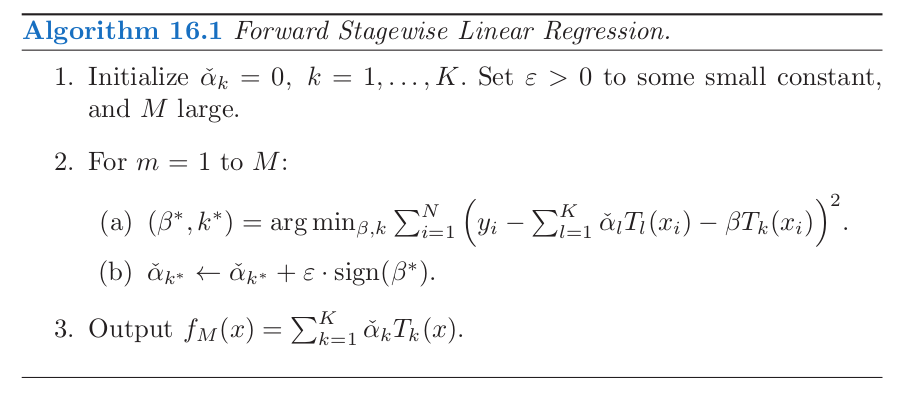
\includegraphics[width=\textwidth]{alg16_1}

(note its similarities with the boosting algorithm)
}

\frame{\frametitle{Ensemble Learning: }
\framesubtitle{boosting and regularization path}
In \textcolor{uio}{comparison} with lasso:
\begin{itemize}
\setlength\itemsep{5pt}
\item initialization ($\textcolor{uio}{\breve{\alpha}_k = 0}, k = 1, \dots, K$) $\longleftrightarrow$ $\textcolor{uio}{\lambda = \infty}$;
\item for \textcolor{uio}{small} values of $M$:
\begin{itemize}
\setlength\itemsep{5pt}
\item some $\breve{\alpha}_k$ are \textcolor{uio}{not updated} $\longleftrightarrow$ coefficients \textcolor{uio}{``forced'' to be 0};
\item $\breve{\alpha}_k^{[0]} \leq \textcolor{uio}{\breve{\alpha}_k^{[M]}} \leq \breve{\alpha}_k^{[\infty]} $ $\longleftrightarrow$ \textcolor{uio}{shrinkage};
\item $M$ \textcolor{uio}{inversely} related to $\lambda$;
\end{itemize}
\item for $M$ large enough ($M=\infty$ in boosting) and $K<N$, $\breve{\alpha}_k^{[M]}= \textcolor{uio}{\hat{\alpha}_{LS}}$ $\textcolor{uio}{\longleftrightarrow}$ $\textcolor{uio}{\lambda = 0}$
\end{itemize}
}


\frame{\frametitle{Ensemble Learning: }
\framesubtitle{boosting and regularization path}
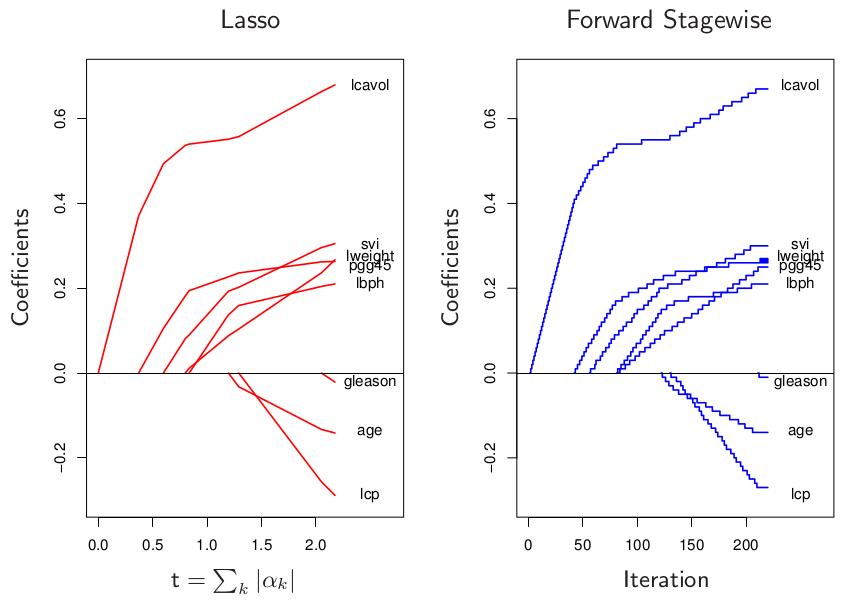
\includegraphics[width=\textwidth]{fig16_1}
}


\frame{\frametitle{Ensemble Learning: }
\framesubtitle{boosting and regularization path}
If
\begin{itemize}
\item all the basis learners $T_K$ are \textcolor{uio}{mutually uncorrelated},
\end{itemize}
then
\begin{itemize}
\item for \textcolor{uio}{$\varepsilon \rightarrow 0$} and \textcolor{uio}{$M\rightarrow \infty$}, such that \textcolor{uio}{$\varepsilon M \rightarrow t$},
\end{itemize}
Algorithm 16.1 gives the \textcolor{uio}{lasso solutions} with \textcolor{uio}{$t = \sum_k |\alpha_k|$}.

\vspace{12pt}

In general component-wise boosting and lasso do \textcolor{uio}{not} provide the same solution:
\begin{itemize}
\item in practice, often \textcolor{uio}{similar in terms of prediction};
\item for $\varepsilon$ ($\nu$) $\rightarrow 0$ \textcolor{uio}{boosting} (and forward stagewise in general) \textcolor{uio}{tends to} the path of the \textcolor{uio}{least angle} regression algorithm;
\item \textcolor{uio}{lasso} can also be seen as a special case of \textcolor{uio}{least angle}.
\end{itemize}
}


\frame{\frametitle{Ensemble Learning: }
\framesubtitle{boosting and regularization path}
Consider 1000 Gaussian distributed variables:
\begin{itemize}
\item \textcolor{uio}{strongly correlated} ($\rho = 0.95$) in blocks of 20;
\item uncorrelated blocks;
\item one variable with effect on the outcome for each block;
\item effects generated from a standard Gaussian.
\end{itemize}

\vspace{12pt}

Moreover:
\begin{itemize}
\item added Gaussian noise;
\item noise-to-signal ratio = 0.72.
\end{itemize}
}


\frame{\frametitle{Ensemble Learning: }
\framesubtitle{boosting and regularization path}
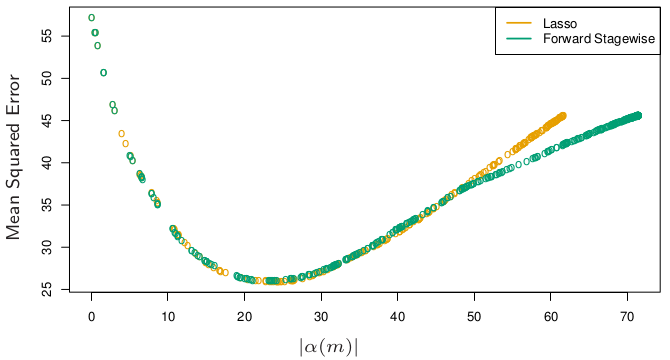
\includegraphics[width=\textwidth]{fig16_4}
}


\frame{\frametitle{Ensemble Learning: }
\framesubtitle{boosting and regularization path}
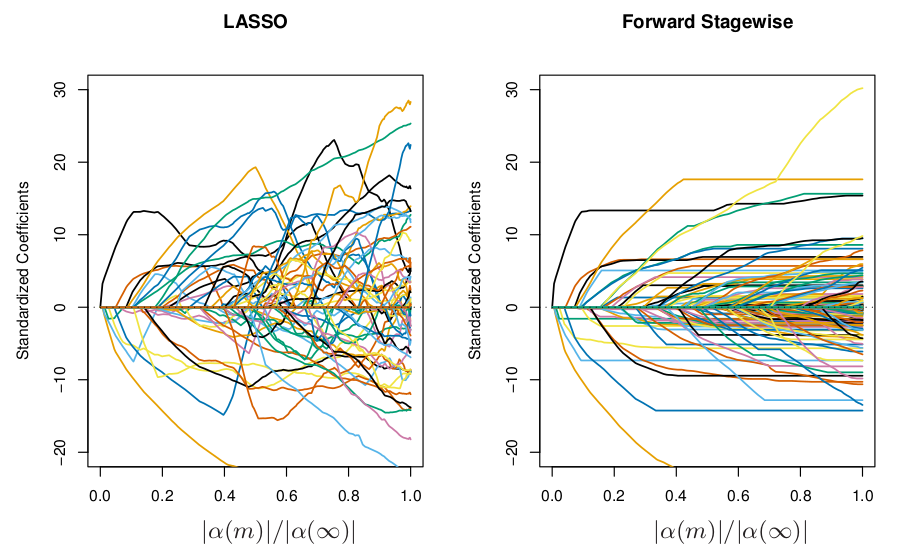
\includegraphics[width=1.05\textwidth]{fig16_3}
}


\subsection{The ``bet on sparsity'' principle}

\frame{\frametitle{Ensemble Learning: }
\framesubtitle{the ``bet on sparsity'' principle}
We consider:
\begin{itemize}
\item \textcolor{uio}{$L_1$-type} of penalty (shrinkage, variable selection);
\item \textcolor{uio}{$L_2$-type} of penalty (shrinkage, computationally easy);
\item boosting's stagewise forward strategy minimizes something \textcolor{uio}{close to} a $L_1$ penalized loss function;
\item step-by-step minimization.
\item[]
\end{itemize}
Can we \textcolor{uio}{characterize} situations where one is preferable to the other?
}

\frame{\frametitle{Ensemble Learning: }
\framesubtitle{the ``bet on sparsity'' principle}
Consider the following framework:
\begin{itemize}
\item 50 observations;
\item 300 independent Gaussian variables.
\end{itemize}

\vspace{12pt}

Three scenarios:
\begin{itemize}
\item \textcolor{uio}{all 300} variables are relevant;
\item \textcolor{uio}{only 10} out of 300 variables are relevant;
\item \textcolor{uio}{30} out of 300 variables are relevant.
\end{itemize}

\vspace{12pt}

Outcome:
\begin{itemize}
\item regression (added standard Gaussian noise);
\item classification (from an inverse-logit transformation of the linear predictor)
\end{itemize}
}


\frame{\frametitle{Ensemble Learning: }
\framesubtitle{the ``bet on sparsity'' principle}
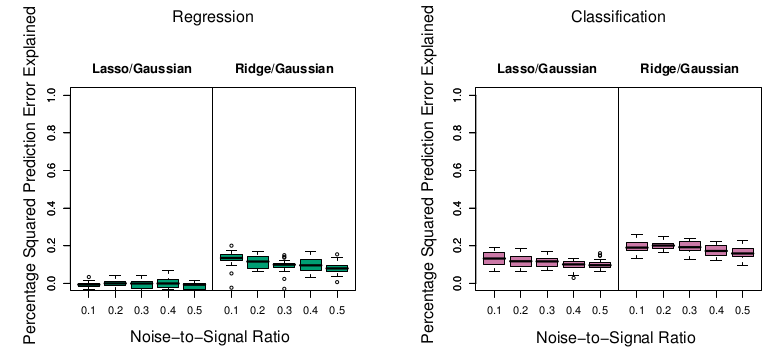
\includegraphics[width=1.05\textwidth]{fig16_2_top}
}


\frame{\frametitle{Ensemble Learning: }
\framesubtitle{the ``bet on sparsity'' principle}
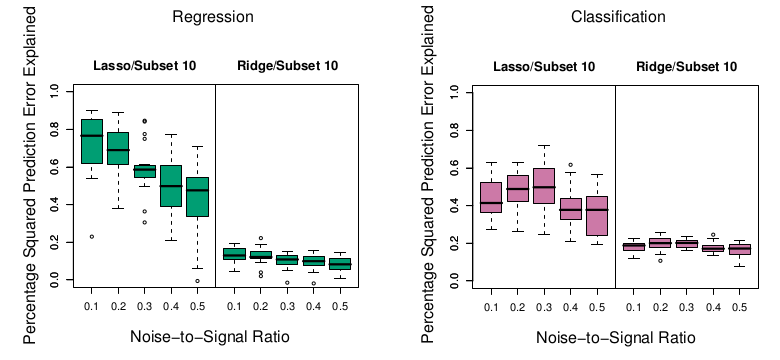
\includegraphics[width=1.05\textwidth]{fig16_2_middle}
}


\frame{\frametitle{Ensemble Learning: }
\framesubtitle{the ``bet on sparsity'' principle}
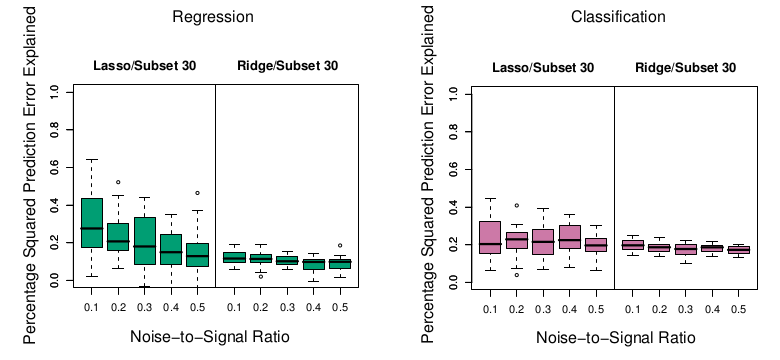
\includegraphics[width=1.05\textwidth]{fig16_2_bottom}
}


\frame{\frametitle{Ensemble Learning: }
\framesubtitle{the ``bet on sparsity'' principle}
This means that:
\begin{itemize}
\item lasso performs \textcolor{uio}{better} than ridge in \textcolor{uio}{sparse} contexts;
\item ridge gives better results if there are \textcolor{uio}{several} relevant variables with \textcolor{uio}{small effects};
\item \textcolor{uio}{anyway}, in the dense case, the model \textcolor{uio}{does not} explain a lot,
\begin{itemize}
\item not enough data to estimate correctly several coefficients;
\end{itemize}
\item[] \centering $\downarrow$
\item[] {\bf ``bet on sparsity''}
\item[] $=$
\item[] \textcolor{uio}{\it ``use a procedure that does well in sparse problems, since no procedure does well in dense problems''}
\end{itemize}
}


\frame{\frametitle{Ensemble Learning: }
\framesubtitle{the ``bet on sparsity'' principle}
The \textcolor{uio}{degree of sparseness} depends on:
\begin{itemize}
\setlength\itemsep{8pt}
\item the \textcolor{uio}{unknown mechanism} generating the data;
\begin{itemize}
\item it depends on the number of relevant variables;
\end{itemize}
\item \textcolor{uio}{size} of the \textcolor{uio}{training set};
\begin{itemize}
\item larger sizes allow estimating denser models;
\end{itemize}
\item \textcolor{uio}{noise-to-signal ratio};
\begin{itemize}
\item smaller NTR $\rightarrow$ denser models (same as before);
\end{itemize}
\item \textcolor{uio}{size} of the \textcolor{uio}{dictionary};
\begin{itemize}
\item more base learners, potentially sparser models.
\end{itemize}\end{itemize}
}



\section{High-Dimensional Problems: $p \gg N$}

\subsection{When $p$ is much larger than $N$}

\frame{\frametitle{High-Dimensional Problems: }
\framesubtitle{when $p$ is much larger than $N$}
The case \textcolor{uio}{$p \gg N$} (number of variable much larger than the number of observations):
\begin{itemize}
\item \textcolor{uio}{very important} in current applications,
\begin{itemize}
\item e.g., in a common genetic study, $p \approx 23000$, $N \approx 100$;
\end{itemize}
\item concerns about \textcolor{uio}{high variance} and \textcolor{uio}{overfitting};
\item \textcolor{uio}{highly regularized approaches} are common:
\begin{itemize}
\item lasso;
\item ridge;
\item boosting;
\item elastic-net;
\item \dots
\end{itemize}
\end{itemize}
}


\frame{\frametitle{High-Dimensional Problems: }
\framesubtitle{when $p$ is much larger than $N$}
Consider the following example:
\begin{itemize}
\item $N = 100$;
\item $p$ variables from standard Gaussians with $\rho = 0.2$,
\begin{center}
$\text{(i) } \textcolor{uio}{p = 10} \quad\quad\quad \text{(ii) } \textcolor{uio}{p = 100} \quad\quad\quad \text{(iii) } \textcolor{uio}{p = 1000}$.
\end{center}

\item response from\\
\begin{center} $Y = \sum_{j=1}^p X_j\beta_j + \sigma\epsilon$; \end{center}
\item signal to noise ratio $\text{Var}[E(Y|X)]/\sigma^2 = 2$;
\item true $\beta$ from a standard Gaussian;
\end{itemize}
}


\frame{\frametitle{High-Dimensional Problems: }
\framesubtitle{when $p$ is much larger than $N$}
As a consequence, averaging over 100 replications:
\begin{itemize}
\item $p_0$, the number of significant $\beta$ (i.e., $\beta : |\hat{\beta}/\hat{\text{se}}|>2$)
\begin{center}
$\text{(i) } \textcolor{uio}{p_0 = 9} \quad\quad\quad \text{(ii) } \textcolor{uio}{p_0 = 33} \quad\quad\quad \text{(iii) } \textcolor{uio}{p_0 = 331}$.
\end{center}
\end{itemize}

\vspace{12pt}

Consider 3 values of the penalty $\lambda$:
\begin{itemize}
\item \textcolor{uio}{$\lambda = 0.001$}, which corresponds to
\begin{center}
$\text{(i) } \text{d.o.f.} = 20 \quad\quad\quad \text{(ii) } \text{d.o.f.} = 99 \quad\quad\quad \text{(iii) } \text{d.o.f.} = 99$;
\end{center}
\item \textcolor{uio}{$\lambda = 100$}, which corresponds to
\begin{center}
$\text{(i) } \text{d.o.f.} = 9 \quad\quad\quad \text{(ii) } \text{d.o.f.} = 35 \quad\quad\quad \text{(iii) } \text{d.o.f.} = 87$;
\end{center}
\item \textcolor{uio}{$\lambda = 1000$}, which corresponds to
\begin{center}
$\text{(i) } \text{d.o.f.} = 2 \quad\quad\quad \text{(ii) } \text{d.o.f.} = 7 \quad\quad\quad \text{(iii) } \text{d.o.f.} = 43$.
\end{center}
\end{itemize}
}

\frame{\frametitle{High-Dimensional Problems: }
\framesubtitle{when $p$ is much larger than $N$}
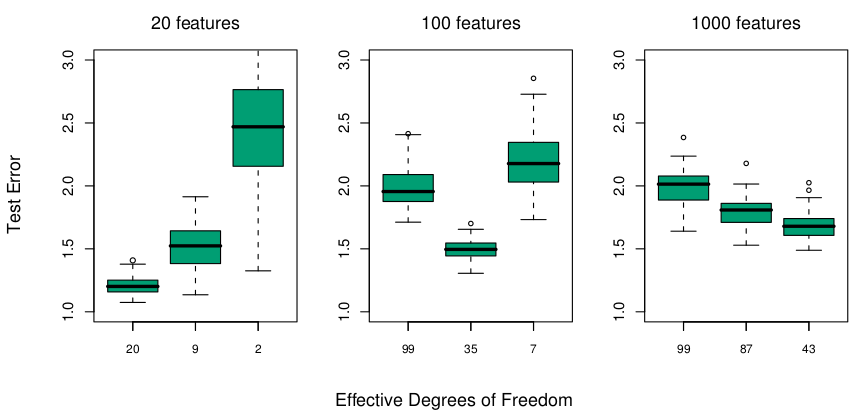
\includegraphics[width=\textwidth]{fig18_1}
}

\frame{\frametitle{High-Dimensional Problems: }
\framesubtitle{when $p$ is much larger than $N$}
Remarks:
\begin{itemize}
\setlength\itemsep{5pt}
\item with \textcolor{uio}{$p=20$}, ridge regression can \textcolor{uio}{find the relevant variables};
\begin{itemize}
\item the covariance matrix can be estimated;
\end{itemize}
\item moderate shrinkage \textcolor{uio}{works better} in the \textcolor{uio}{middle case}, in which we can find some non-zero effects;
\item with \textcolor{uio}{$p=1000$}, there is \textcolor{uio}{no hope to find} the relevant variables, and it is better to \textcolor{uio}{shrink down everything};
\begin{itemize}
\item no possibility to estimate the covariance matrix.
\end{itemize}
\end{itemize}
}


\subsection{Computational short-cuts when $p\gg N$}

\frame{\frametitle{High-Dimensional Problems: }
\framesubtitle{computational short-cuts when $p\gg N$}
Consider the \textcolor{uio}{single-value decomposition} of X,
\begin{align*}
X &= UDV^T\\
 &= RV^T
\end{align*}
Where
\begin{itemize}
\item $V$ is a $p\times N$ matrix with orthonormal columns;
\item $U$ is a $N\times N$ orthonormal matrix;
\item $D$ is a diagonal matrix with elements $d_1 \geq d_2 \geq \dots \geq d_N \geq 0$;
\item $R$ is a $N\times N$ with rows $r_i$.
\end{itemize}
}


\frame{\frametitle{High-Dimensional Problems: }
\framesubtitle{computational short-cuts when $p\gg N$}
{\it Theorem \citep[][page 660]{HastieAl2009}:}

Let $f^*(r_i) = \theta_0 + r_i^T\theta$ and consider the optimization problems:
\begin{align*}
(\hat{\beta}_0, \hat{\beta}) &= \text{argmin}_{\beta_0, \beta \in \mathds{R}^p} \sum_{i=1}^N L(y_i, \beta_0 + x_i\beta) + \lambda\beta^T\beta;\\
(\hat{\theta}_0, \hat{\theta}) &= \text{argmin}_{\theta_0, \theta \in \mathds{R}^N} \sum_{i=1}^N L(y_i, \theta_0 + r_i\theta) + \lambda\theta^T\theta.
\end{align*}
Then \textcolor{uio}{$\beta_0 = \theta_0$} and \textcolor{uio}{$\hat{\beta} = V\hat{\theta}$}.
}

\frame{\frametitle{High-Dimensional Problems: }
\framesubtitle{computational short-cuts when $p\gg N$}
Note:
\begin{itemize}
\item we can replace the \textcolor{uio}{$p$-dim} vectors $x_i$ with the \textcolor{uio}{$N$-dim} vectors $r_i$;
\item same penalization, but with \textcolor{uio}{way fewer predictors};
\item the $N$-dimensional solution $\hat{\theta}$ is transformed back to the $p$-dimensional $\hat{\beta}$ by \textcolor{uio}{simple matrix multiplication};
\item it only works for \textcolor{uio}{linear models};
\item it only works for \textcolor{uio}{quadratic penalties}.
\item[]
\item a \textcolor{uio}{$O(p^3)$} problem is reduced to a \textcolor{uio}{$O(p^2N)$} problem;
\begin{itemize}
\item relevant for $p > N$.
\end{itemize}
\end{itemize}
}

\frame{\frametitle{High-Dimensional Problems: }
\framesubtitle{computational short-cuts when $p\gg N$}
{\it Example (ridge regression):}

Consider the estimate of a ridge regression,
$$
\hat{\beta} = (X^TX + \lambda I)^{-1}X^Ty.
$$
Replacing $X$ with $RV^T$, we obtain
$$
\hat{\beta} = V(R^TR + \lambda I)^{-1}R^Ty,
$$
i.e.,
$$
\textcolor{uio}{\hat{\beta} = V \hat{\theta}},
$$
where
$$
\hat{\theta} = (R^TR + \lambda I)^{-1}R^Ty.
$$
}

\frame{\frametitle{High-Dimensional Problems: }
\framesubtitle{computational short-cuts when $p\gg N$}
Note:
\begin{itemize}
\item it \textcolor{uio}{cannot} be applied to \textcolor{uio}{lasso};
\item the short-cut is particularly \textcolor{uio}{relevant for} finding the best $\lambda$ via \textcolor{uio}{cross-validation};
\item it can be shown that one need to construct $R$ only once,
\begin{itemize}
\item use the same $R$ for each of the CV-folds.
\end{itemize}
\end{itemize}
}


\subsection{Supervised Principal Component}

\frame{\frametitle{High-Dimensional Problems: }
\framesubtitle{supervised principal component}
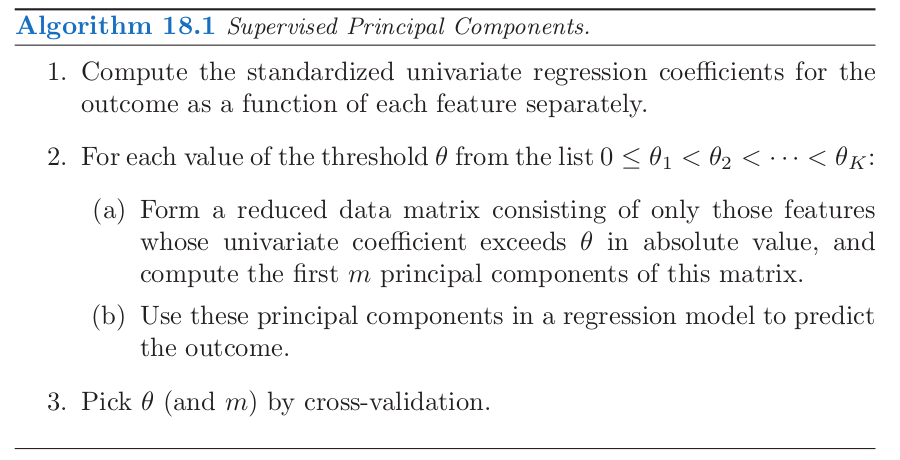
\includegraphics[width=\textwidth]{alg18_1}
}

\frame{\frametitle{High-Dimensional Problems: }
\framesubtitle{supervised principal component}
Note:
\begin{itemize}
\setlength\itemsep{5pt}
\item in the first step, the variables \textcolor{uio}{univariately most associated} with the outcome are selected:
\begin{itemize}
\item the measure depends on the \textcolor{uio}{nature of the outcome};
\item include all associations larger than a \textcolor{uio}{threshold $\theta$};
\item may include \textcolor{uio}{highly correlated} variables.
\end{itemize}
\item in step 2, \textcolor{uio}{perform PCR} on the reduced variable space:
\begin{itemize}
\item use the \textcolor{uio}{first $m$ components};
\item assure \textcolor{uio}{shrinkage}.
\end{itemize}
\item both $\theta$ and $m$ \textcolor{uio}{must be computed} by cross-validation:
\begin{itemize}
\item \textcolor{uio}{2-dimension} tuning parameter.
\end{itemize}
\end{itemize}
}

\frame{\frametitle{High-Dimensional Problems: }
\framesubtitle{supervised principal component}
Example (survival analysis with microarray data):
\begin{itemize}
\item data from \cite{RosenwaldAl2002};
\item input: 7399 gene expressions of 240 patients;
\item response: survival time (potentially right censored);
\item divided in a training (160 patients) and (80) test set.
\end{itemize}
\centering
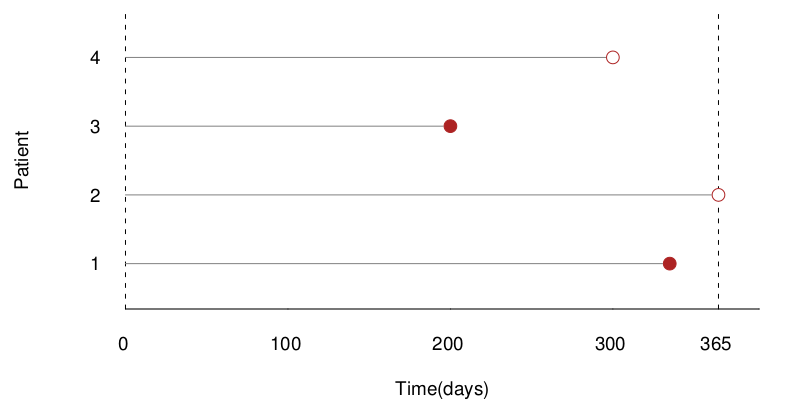
\includegraphics[width=0.75\textwidth]{fig18_11}
}

\frame{\frametitle{High-Dimensional Problems: }
\framesubtitle{supervised principal component}
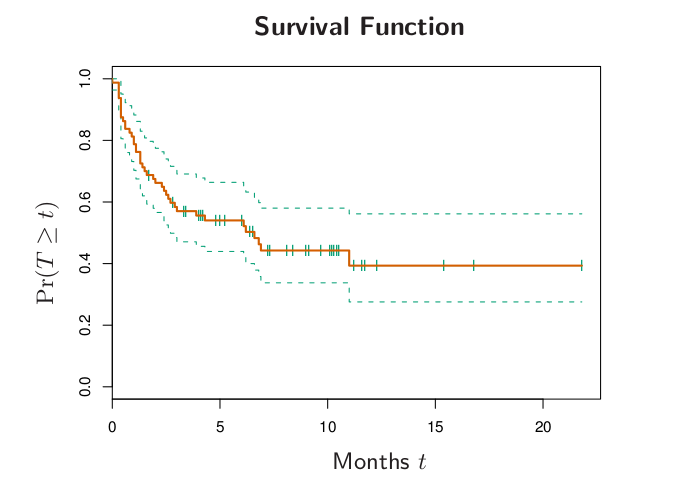
\includegraphics[width=\textwidth]{fig18_12}
}

\frame{\frametitle{High-Dimensional Problems: }
\framesubtitle{supervised principal component}
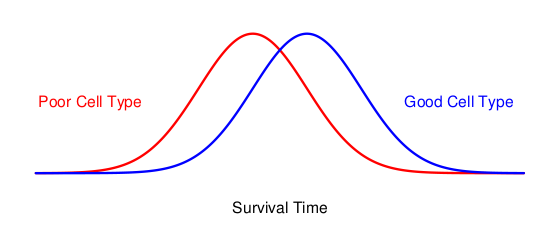
\includegraphics[width=\textwidth]{fig18_13}
}

\frame{\frametitle{High-Dimensional Problems: }
\framesubtitle{supervised principal component}
\centering
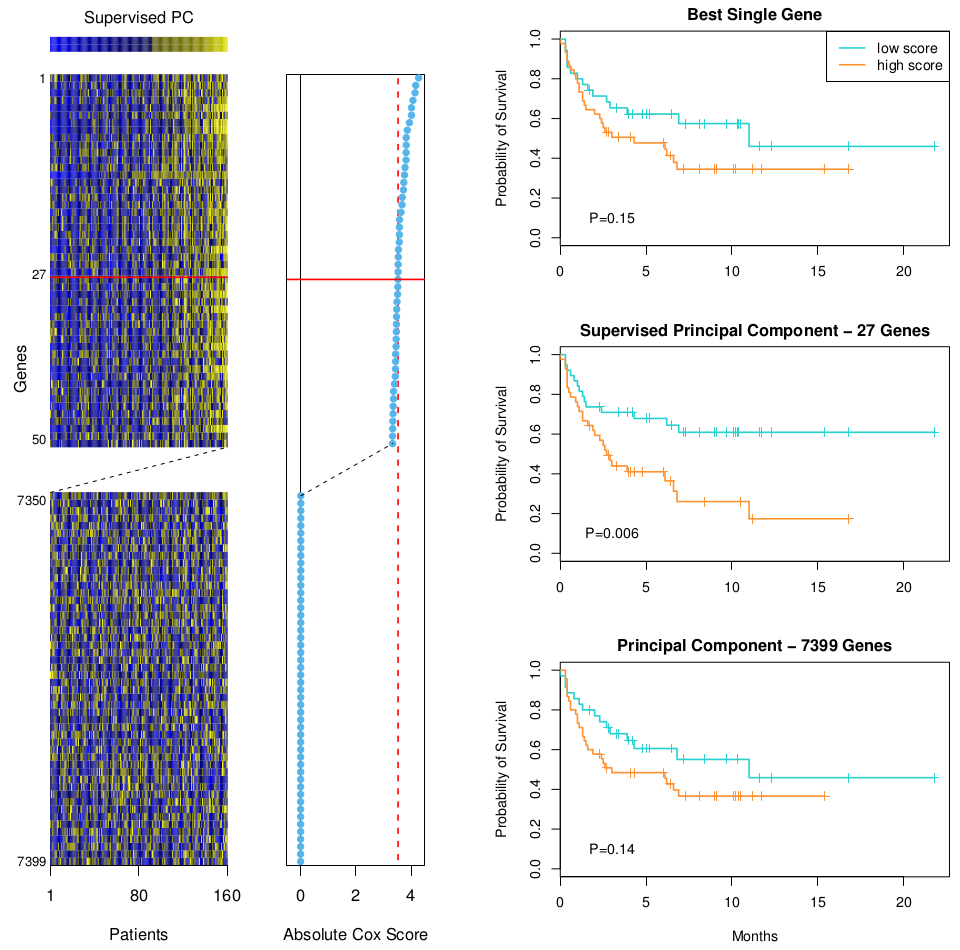
\includegraphics[width=0.7\textwidth]{fig18_14}
}

\frame{\frametitle{High-Dimensional Problems: }
\framesubtitle{supervised principal component}
\centering
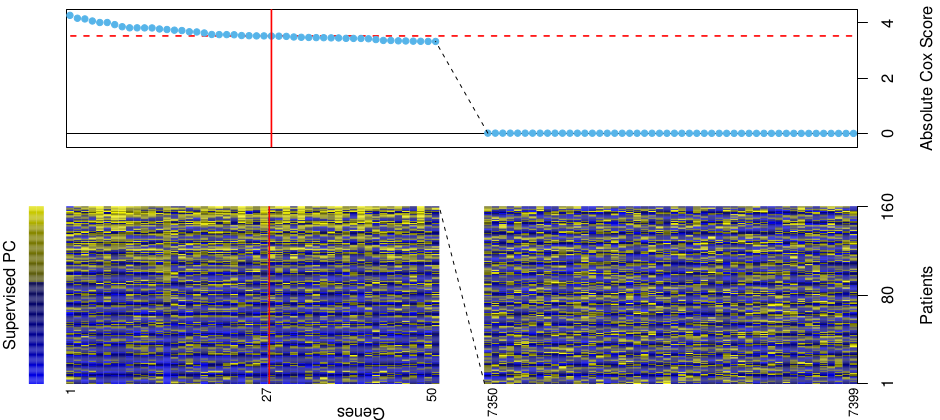
\includegraphics[width=1.05\textwidth]{fig18_14_left}
}

\frame{\frametitle{High-Dimensional Problems: }
\framesubtitle{supervised principal component}
\centering
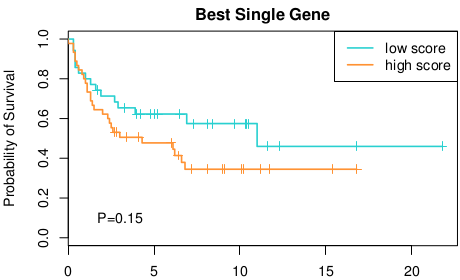
\includegraphics[width=0.5\textwidth]{fig18_14_rt}
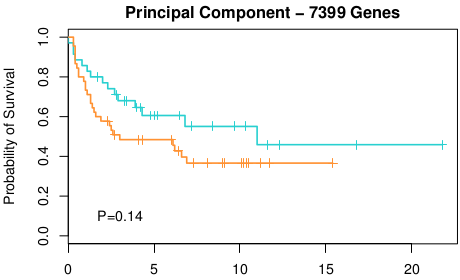
\includegraphics[width=0.5\textwidth]{fig18_14_rb}\\
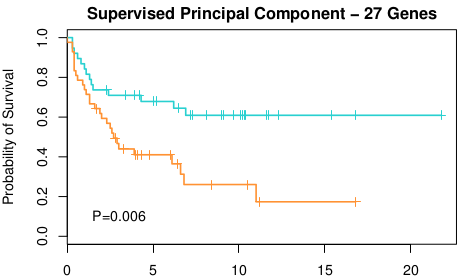
\includegraphics[width=0.5\textwidth]{fig18_14_rm}
}

\frame{\frametitle{High-Dimensional Problems: }
\framesubtitle{supervised-PC and latent-variable modelling}
Consider a {\bf \uline{latent-variable model}},
$$
Y = \beta_0 + \beta_1U + \epsilon
$$
where
$$
X_j = \alpha_{0j} + \alpha{1j}U + \epsilon_j \quad\quad \textcolor{uio}{\text{ if } j \in \mathcal{P}}
$$
\begin{itemize}
\item $\epsilon$ and $\epsilon_j$ have \textcolor{uio}{mean 0} and they are \textcolor{uio}{independent} of the other variables in their respective models;
\item $X_j$ are \textcolor{uio}{independent} of $U$ if \textcolor{uio}{$j \notin \mathcal{P}$}.
\end{itemize}
}

\frame{\frametitle{High-Dimensional Problems: }
\framesubtitle{supervised-PC and latent-variable modelling}
Supervised-PC can be seen as a method to fit this kind of model:
\begin{itemize}
\setlength\itemsep{5pt}
\item step 1: \textcolor{uio}{identify} the $j \in \mathcal{P}$;
\begin{itemize}
\item on average $\beta_1$ is not zero only if $\alpha_{1j} \neq 0$;
\end{itemize}
\item step 2a: \textcolor{uio}{estimate} $\alpha_{0j}$ and $\alpha_{1j}$
\begin{itemize}
\item natural if $\epsilon_j \sim N(0;\sigma^2)$;
\end{itemize}
\item step 2b: estimate $\beta_0$ and $\beta_1$ (\textcolor{uio}{fit the model}).
\end{itemize}
}

\frame{\frametitle{High-Dimensional Problems: }
\framesubtitle{supervised-PC and partial least square}
Supervised-PC versus \textcolor{uio}{partial least square}:
\begin{itemize}
\item both aim at considering both \textcolor{uio}{large variation} and \textcolor{uio}{correlation with the outcome};
\item supervised-PC \textcolor{uio}{removes} those which are not relevant;
\item partial least square \textcolor{uio}{downgrades} them
\item[] $\quad\quad\quad\downarrow$
\item[] ``thresholded PLS'':
\begin{itemize}
\item apply PLS on \textcolor{uio}{only} the variables selected by supervised-PC.
\end{itemize}
\end{itemize}
}

\frame{\frametitle{High-Dimensional Problems: }
\framesubtitle{supervised-PC and partial least square}
Thresholded PLS can be seen as a \textcolor{uio}{noisy version} of supervised-PC,
\begin{itemize}
\item first \textcolor{uio}{PLS variate}, \begin{center}$z = \sum_{j \in \mathcal{P}} \langle y,x_j\rangle x_j$;\end{center}
\item \textcolor{uio}{supervised principal component direction}, \begin{center}$u = \frac{1}{d^2} \sum_{j \in \mathcal{P}} \langle y,x_j\rangle x_j$.\end{center}
\end{itemize}

\vspace{12pt}

Set $p_1 = |\mathcal{P}|$. It can be shown \citep{BairTibshirani2004} that, for $N, p_1, p \rightarrow \infty$, s.t.\ $p_1/N \rightarrow 0$
\textcolor{uio}{\begin{align*}
z &= u + O_p(1)\\
\hat{u} &= u + O_p(\sqrt{p_1/N})
\end{align*}}
where $u$ is the true latent variable.
}


\frame{\frametitle{High-Dimensional Problems: }
\framesubtitle{supervised-PC and partial least square}
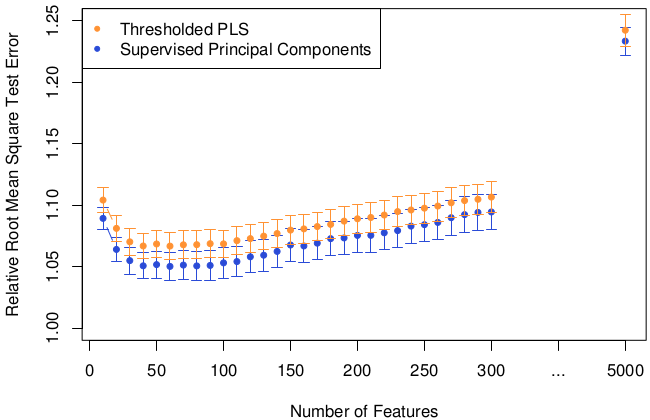
\includegraphics[width=\textwidth]{fig18_16}
}


\frame{\frametitle{High-Dimensional Problems: }
\framesubtitle{pre-conditioning}
Supervised-PC can also be used to \textcolor{uio}{improve lasso} performance, through pre-conditioning
\begin{itemize}
\item compute $\hat{y}_i$ the \textcolor{uio}{supervised-PC prediction} for each observation;
\item apply lasso using \textcolor{uio}{$\hat{y}_i$ instead of $y_i$} as outcome;
\begin{itemize}
\item using \textcolor{uio}{all} variables, not only those selected by supervised-PC.
\end{itemize}
\item[]
\end{itemize}
The idea is to \textcolor{uio}{remove the noise}, so lasso is \textcolor{uio}{not affected} by the large number of noisy variables.
}


\frame{\frametitle{High-Dimensional Problems: }
\framesubtitle{pre-conditioning}
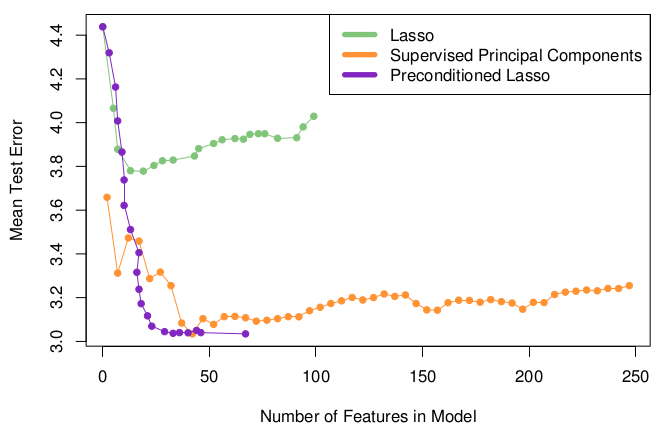
\includegraphics[width=\textwidth]{fig18_17}
}


%%%%%%%%%%%
\section*{Bibliography}
%%%%%%%%%%%

\frame[allowframebreaks]{\frametitle{References}
\footnotesize
\bibliographystyle{../../../../support/biometrika}
\bibliography{../../../../support/biblio}
}

\end{document}
